\documentclass[12pt,a4paper,oneside,DIV=14]{scrartcl}
\usepackage[utf8]{inputenc}
\usepackage[ngerman]{babel}
\usepackage[T1]{fontenc}
\usepackage[sc,osf]{mathpazo} 
\usepackage{nag}
\usepackage{graphicx}
\usepackage{caption}
\usepackage[]{enumitem}
\usepackage{multicol}

\setlist{itemsep=-5pt}


%% Einstellungen aus Template
\newcommand{\mycolorlinks}{true}
\newcommand{\myauthor}{Lukas Winkler}
\newcommand{\mytitle}{Begleitprotokoll -- Umweltdatenmessung mit dem Raspberry Pi} 
\newcommand{\mysubject}{\mytitle}
\newcommand{\mykeywords}{Umweltdatenmessung, Raspberry, Temperatur, Klimadaten, Wetter, Auswertung, Software}

\usepackage{xcolor}
\definecolor{DispositionColor}{RGB}{30,103,182}
%%%% Time-stamp: <2014-03-23 13:40:59 vk>
%%%% === Disclaimer: =======================================================
%% created by
%%
%%      Karl Voit
%%
%% using GNU/Linux, GNU Emacs & LaTeX 2e
%%

%doc%
%doc% \section{\texttt{pdf\_settings.tex} --- Settings related to PDF output}
%doc% \label{sec:pdf}
%doc% 
%doc% The file \verb#template/pdf_settings.tex# basically contains the definitions for
%doc% the \href{http://tug.org/applications/hyperref/}{\texttt{hyperref} package}
%doc% including the
%doc% \href{http://www.ctan.org/tex-archive/macros/latex/required/graphics/}{\texttt{graphicx}
%doc% package}. Since these settings should be the last things of any \LaTeX{}
%doc% preamble, they got their own \TeX{} file which is included in \texttt{main.tex}.
%doc% 
%doc% \paragraph{What should I do with this file?} The settings in this file are
%doc% important for \myacro{PDF} output and including graphics. Do not exclude the
%doc% related \texttt{input} command in \texttt{main.tex}. But you might want to
%doc% modify some settings after you read the
%doc% \href{http://tug.org/applications/hyperref/}{documentation of the \texttt{hyperref} package}.
%doc% 


%% Fix positioning of images in PDF viewers. (disabled by
%% default; see https://github.com/novoid/LaTeX-KOMA-template/issues/4
%% for more information) 
%% I do not have time to read about possible side-effect of this
%% package for now.
% \usepackage[hypcap]{caption}

%% Declarations of hyperref should be the last definitions of the preamble:
%% FIXXME: black-and-white-version for printing!

\pdfcompresslevel=9

\usepackage[%
unicode=true, % loads with unicode support
%a4paper=true, %
pdftex=true, %
backref, %
pagebackref=false, % creates backward references too
bookmarks=false, %
bookmarksopen=false, % when starting with AcrobatReader, the Bookmarkcolumn is opened
pdfpagemode=None,% None, UseOutlines, UseThumbs, FullScreen
plainpages=false, % correct, if pdflatex complains: ``destination with same identifier already exists''
%% colors: https://secure.wikimedia.org/wikibooks/en/wiki/LaTeX/Colors
urlcolor=DispositionColor, %%
linkcolor=DispositionColor, %%
pagecolor=DispositionColor, %%
citecolor=DispositionColor, %%
anchorcolor=DispositionColor, %%
colorlinks=\mycolorlinks, % turn on/off colored links (on: better for
                          % on-screen reading; off: better for printout versions)
]{hyperref}

%% all strings need to be loaded after hyperref was loaded with unicode support
%% if not the field is garbled in the output for characters like ČŽĆŠĐ
\hypersetup{
pdftitle={\mytitle}, %
pdfauthor={\myauthor}, %
pdfsubject={\mysubject}, %
pdfcreator={Accomplished with: pdfLaTeX, biber, and hyperref-package. No animals, MS-EULA or BSA-rules were harmed.},
pdfproducer={\myauthor},
pdfkeywords={\mykeywords}
}

%\DeclareGraphicsExtensions{.pdf}

%%%% END
%%% Local Variables:
%%% TeX-master: "../main"
%%% mode: latex
%%% mode: auto-fill
%%% mode: flyspell
%%% eval: (ispell-change-dictionary "en_US")
%%% End:
%% vim:foldmethod=expr
%% vim:fde=getline(v\:lnum)=~'^%%%%'?0\:getline(v\:lnum)=~'^%doc.*\ .\\%(sub\\)\\?section{.\\+'?'>1'\:'1':

\hyphenpenalty=3000 
\tolerance=1000

\author{\myauthor}
\title{Begleitprotokoll}
\subtitle{Umweltdatenmessung mit dem Raspberry Pi}
\begin{document}
\maketitle

\section{Verlauf -- Kontakt mit Betreuungslehrer}
\begin{multicols}{2}
\begin{itemize}

	\item Sommerferien 2013:
	\begin{itemize}
		\item kaufen eines \emph{Raspberry Pi}
		\item experimentieren, testen der Möglichkeiten
	\end{itemize}
	\item September/Oktober 2013:
	\begin{itemize}
		\item eine der ersten Informatik-Stunden: suchen nach Raspberry Pi-Projekten für den Unterricht\newline Idee, eine Wetterstation zu bauen.
		\item bis zur nächsten Stunde: schreiben eines Programmes, welches zufällige Datenreihen erstellt und als Diagramm grafisch darstellt.
	\end{itemize}
	\item 14. Oktober 2013
	\begin{itemize}
		\item einrichten einer Webseite\footnote{\href{http://lukaswiki.onpw.de/rasp/}{lukaswiki.onpw.de/rasp} (nicht mehr erreichbar, Kopie unter \href{http://winkler.kremszeile.at/rasp/}{winkler.kremszeile.at/rasp})}, auf der alle Dateien und Fortschritte protokolliert werden.
	\end{itemize}
	\item 2. November 2013
	\begin{itemize}
		\item erste Teile für die Hardware gekauft (Steckbrett, Verbindungskabel, Temperatursensor)
	\end{itemize}
	\item 14. November 2013
	\begin{itemize}
		\item erste erfolgreiche Messung
	\end{itemize}
	\item 19. November 2013
	\begin{itemize}
		\item erstes Display funktioniert
	\end{itemize}
	\item Dezember 2013
	\begin{itemize}
		\item Messung über zwei Wochen
	\end{itemize}
	\item 20. Dezember 2013
	\begin{itemize}
		\item Treffen mit Betreuungslehrer, Besprechung des aktuellen Zwischenstandes
	\end{itemize}
	\item 27. Dezember 2013
	\begin{itemize}
		\item komplette Projekt ist auf Github\footnote{\href{https://github.com/Findus23/Umweltdatenmessung}{github.com/Findus23/Umweltdatenmessung}} (Versionsverwaltung)
	\end{itemize}
	\item 15. Jänner 2014
	\begin{itemize}
		\item Besprechung der Einreichung mit dem Betreuungslehrer
		\item einreichen der Themenstellung
	\end{itemize}
	\item Jänner 2014
	\begin{itemize}
		\item zusätzliche Sensoren: Luftdruck und Luftfeuchtigkeit
	\end{itemize}
	\item Anfang Februar 2014
	\begin{itemize}
		\item Stabiles Gehäuse für Messtation.
		\item Bericht des Zwischenstandes an den Betreuungslehrer per E-Mail
	\end{itemize}
	\item Ende Februar 2014
	\begin{itemize}
		\item Luftqualitätssensor
	\end{itemize}
	\item April 2014
	\begin{itemize}
		\item Weboberfläche grundlegend verbessert (Anzeige der Live-Werte)
	\end{itemize}
	\item 23. April 2014
	\begin{itemize}
		\item Präsentation bei den \textsf{EDU|days}\footnote{\href{http://www.edudays.at/}{www.edudays.at}}
	\end{itemize}
	\item 17. Juni 2014
	\begin{itemize}
		\item Sieg im Finale vom \textsf{computer creative wettbewerb} des OCG
	\end{itemize}
	\item Sommer 2014
	\begin{itemize}
		\item Artikel im OCG Journal\footnote{\href{http://www.ocg.at/sites/ocg.at/files/medien/pdfs/OCG-Journal1403.pdf}{OCG Journal 3/2014: Seite 33}}
	\end{itemize}
	\item 19. September 2014
	\begin{itemize}
		\item Beginn mit dem Schreiben der VWA
	\end{itemize}
	\item 6. Oktober 2014
	\begin{itemize}
		\item Präsentation beim 3. IKT-Konvent (Arbeitskreis \emph{Bildung, Wissenschaft und Forschung}
	\end{itemize}
	\item Anfang Jänner
	\begin{itemize}
		\item Besprechung mit Betreuungslehrer über Fertigstellen der VWA
	\end{itemize}
	\item Semesterferien
	\begin{itemize}
		\item Fertigstellen der VWA und abschließende Kommunikation mit Betreuungslehrer
	\end{itemize}		
\end{itemize}
\end{multicols}
\begin{figure}[h]
  \centering
     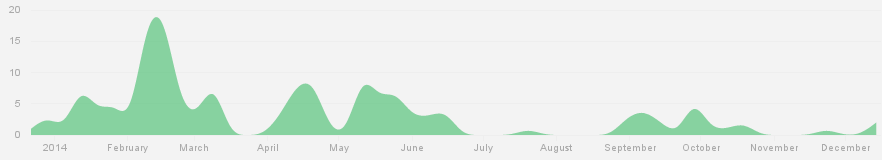
\includegraphics[width=\textwidth]{figures/github_verlauf}
  \caption*{Verlauf der Software-Änderungen (Github)}
  \label{fig:github}
\end{figure}

\section{Länge der Arbeit}
\begin{table}[h]
	\centering
	\label{länge}
	\begin{tabular}{c|c|c|c}
	Teil		&	\LaTeX-Code & \LaTeX\ ohne Befehle (detex) & PDF \\
	\hline\hline
	Einleitung	& 1461 & 1317 & 1161\\\hline
	Hardware	 & 11538	 & 8791 & 6848\\\hline
	Software	& 15142 & 12770 & 14575	\\ \hline
	Auswertung & 4192 & 3360 & 2313 \\ \hline
	Fazit & 2299 & 2121 & 1808 \\ \hline\hline

	Gesamt	& 34632  & 28359 & 26705 \\ \hline\hline
	
	Weitere Informationen & 1190 & 1020 & 812 \\ \hline
	Präsentationen & 2299 & 1989 & 1068 \\ \hline
	Literaturverzeichnis & --- & --- & 5151 \\\hline
	Abstract & 1184 & 1159 & 1123 \\\hline
	Glosar & 5483 & 4290 & 3336 \\ \hline	\hline
	komplette PDF & --- & --- & 51241 \\
	\end{tabular}
\end{table}
\end{document}
